% Security threat model & assumption-ledger dependency graph — for §6.
% Grounded in 055-security.tex: threat model (PPT adversary, malicious prover/verifier)
% and the A1-A8 ledger, each graded established / empirical / open. Arrows show which
% assumptions the preservation theorem depends on; colour = status.
% Compile: pdflatex threat_model.tex
\documentclass[border=4pt]{standalone}
\usepackage{tikz}
\usepackage{newtxtext,newtxmath}
\usetikzlibrary{positioning,arrows.meta,fit,backgrounds,calc}
\begin{document}
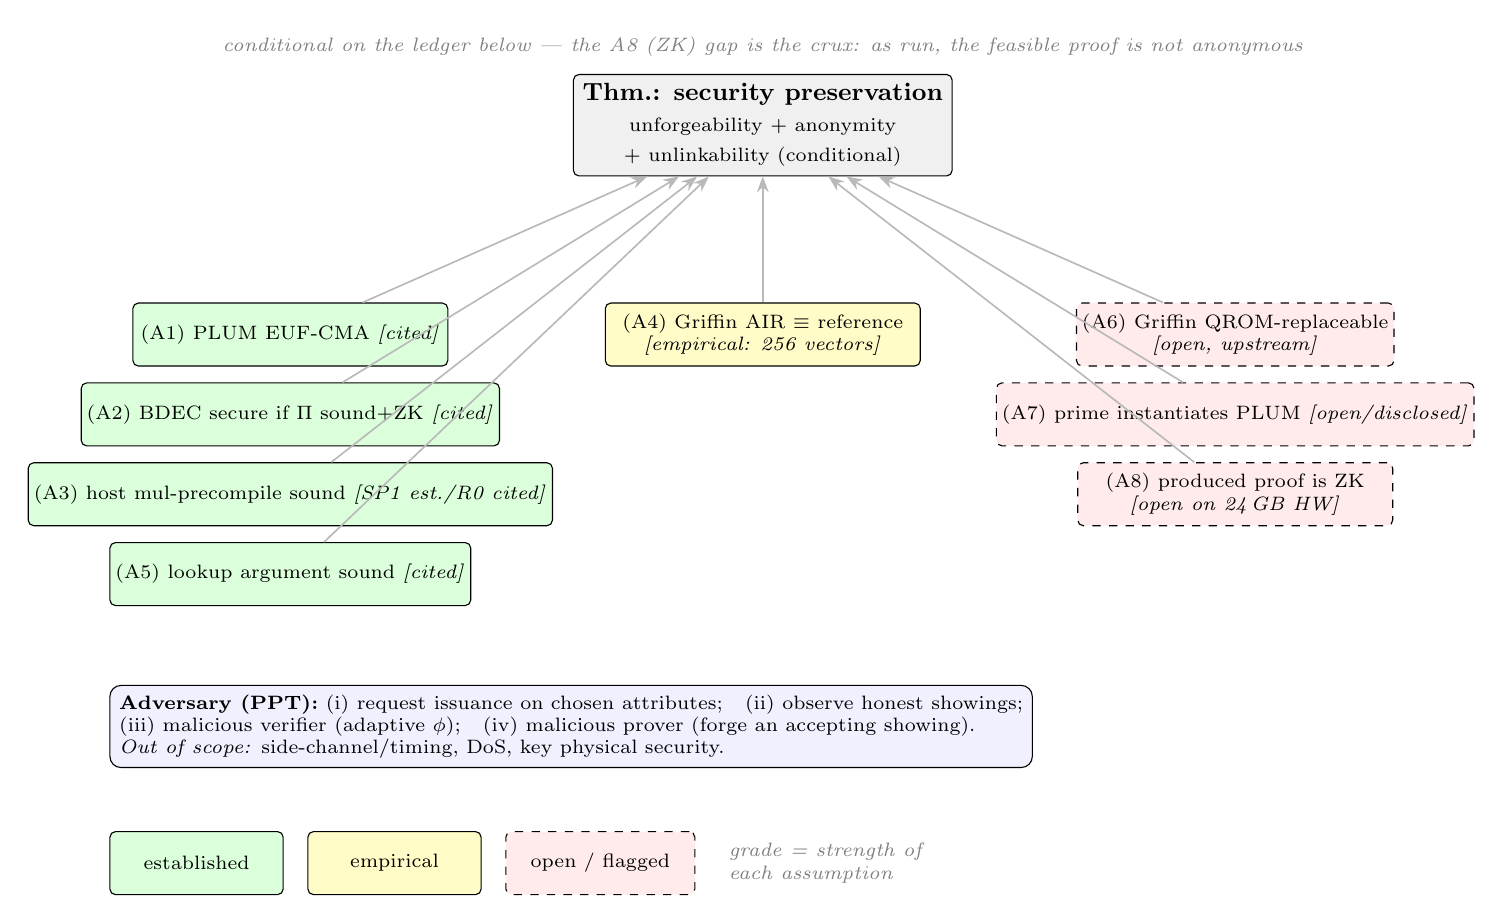
\begin{tikzpicture}[
  font=\small,>={Stealth[length=2mm]},
  thm/.style={draw,rounded corners=2pt,fill=gray!12,minimum width=46mm,minimum height=12mm,align=center},
  est/.style={draw,rounded corners=2pt,fill=green!14,minimum width=40mm,minimum height=8mm,inner sep=2pt,font=\scriptsize,align=center},
  emp/.style={draw,rounded corners=2pt,fill=yellow!22,minimum width=40mm,minimum height=8mm,inner sep=2pt,font=\scriptsize,align=center},
  opn/.style={draw,dashed,rounded corners=2pt,fill=red!8,minimum width=40mm,minimum height=8mm,inner sep=2pt,font=\scriptsize,align=center},
  lbl/.style={font=\scriptsize\itshape,gray},
  dep/.style={->,semithick,gray!55},
]
% theorem at the top
\node[thm] (thm) {\textbf{Thm.: security preservation}\\\scriptsize unforgeability + anonymity\\\scriptsize + unlinkability (conditional)};

% established (left column)
\node[est,below=16mm of thm,xshift=-60mm] (a1) {(A1) PLUM EUF-CMA \emph{[cited]}};
\node[est,below=2mm of a1]                (a2) {(A2) BDEC secure if $\Pi$ sound+ZK \emph{[cited]}};
\node[est,below=2mm of a2]                (a3) {(A3) host mul-precompile sound \emph{[SP1 est./R0 cited]}};
\node[est,below=2mm of a3]                (a5) {(A5) lookup argument sound \emph{[cited]}};

% empirical (centre)
\node[emp,below=16mm of thm,xshift=0mm]   (a4) {(A4) Griffin AIR $\equiv$ reference\\\emph{[empirical: 256 vectors]}};

% open (right column)
\node[opn,below=16mm of thm,xshift=60mm]  (a6) {(A6) Griffin QROM-replaceable\\\emph{[open, upstream]}};
\node[opn,below=2mm of a6]                (a7) {(A7) prime instantiates PLUM \emph{[open/disclosed]}};
\node[opn,below=2mm of a7]                (a8) {(A8) produced proof is ZK\\\emph{[open on 24\,GB HW]}};

% dependency arrows
\foreach \a in {a1,a2,a3,a5,a4,a6,a7,a8} \draw[dep] (\a) -- (thm);

% adversary box — anchored below a5 (the lowest left-column box) so it clears all rows
\node[draw,rounded corners,fill=blue!6,font=\scriptsize,align=left,
      below=10mm of a5.south west,anchor=north west] (adv)
  {\textbf{Adversary (PPT):} (i) request issuance on chosen attributes;\quad
   (ii) observe honest showings;\\
   (iii) malicious verifier (adaptive $\phi$);\quad
   (iv) malicious prover (forge an accepting showing).\\
   \emph{Out of scope:} side-channel/timing, DoS, key physical security.};

% legend
\node[est,below=8mm of adv.south west,anchor=north west,minimum width=22mm] (le) {established};
\node[emp,right=3mm of le,minimum width=22mm] (lp) {empirical};
\node[opn,right=3mm of lp,minimum width=24mm] (lo) {open / flagged};
\node[lbl,right=3mm of lo,align=left] {grade = strength of\\each assumption};

\node[lbl,above=1mm of thm,align=center] {conditional on the ledger below --- the A8 (ZK) gap is the crux: as run, the feasible proof is not anonymous};
\end{tikzpicture}
\end{document}
